\documentclass{beamer}

\usepackage[utf8]{inputenc} 
\usepackage[T1]{fontenc}
\usepackage{lmodern}
\usepackage{graphicx}
\usepackage[french]{babel}
\usepackage{multimedia}

\usetheme{Hannover}
\usecolortheme{crane}
 
\title{Aide'Gare}
\subtitle{Un aperçu technique}
\author{Julia Dirand, Etienne Membrives, Alexandre Rieux}
\institute{Hackcess Angels}
\date{19 septembre 2014} 

\AtBeginSection[] {
  \begin{frame}<beamer>{Lignes directrices}
    \begin{small}
      \tableofcontents[currentsection]
    \end{small}
  \end{frame}
}

\begin{document}
\begin{frame}
  \titlepage
\end{frame}

\begin{frame}{Lignes directrices}
  \setcounter{tocdepth}{3} % Dans la table des matieres
  \tableofcontents
  % Vous pouvez, si vous le souhaiter ajouter l'option [pausesections]
\end{frame}

\section{Quelles spécifications?}
\subsection{Spécifications fonctionnelles}
\begin{frame}{Les demandes générales}
    \begin{block}{Du hackathon}
		\begin{itemize}
			\item Un système simple
			\item Fonctionne dans le plus de situations possibles
		\end{itemize}
    \end{block}
    \begin{block}{Des associations}
		\begin{itemize}
			\item Simplicité d'usage
			\item Information en continu
		\end{itemize}
    \end{block}
    \begin{block}{De la SNCF}
		\begin{itemize}
			\item Sécuriser les agents (collecte de données, formation)
			\item Limiter les demandes (prévenir l'usager des limites)
		\end{itemize}
	\end{block}
\end{frame}
 
\begin{frame}{La demande d'aide}
    \begin{centering}
        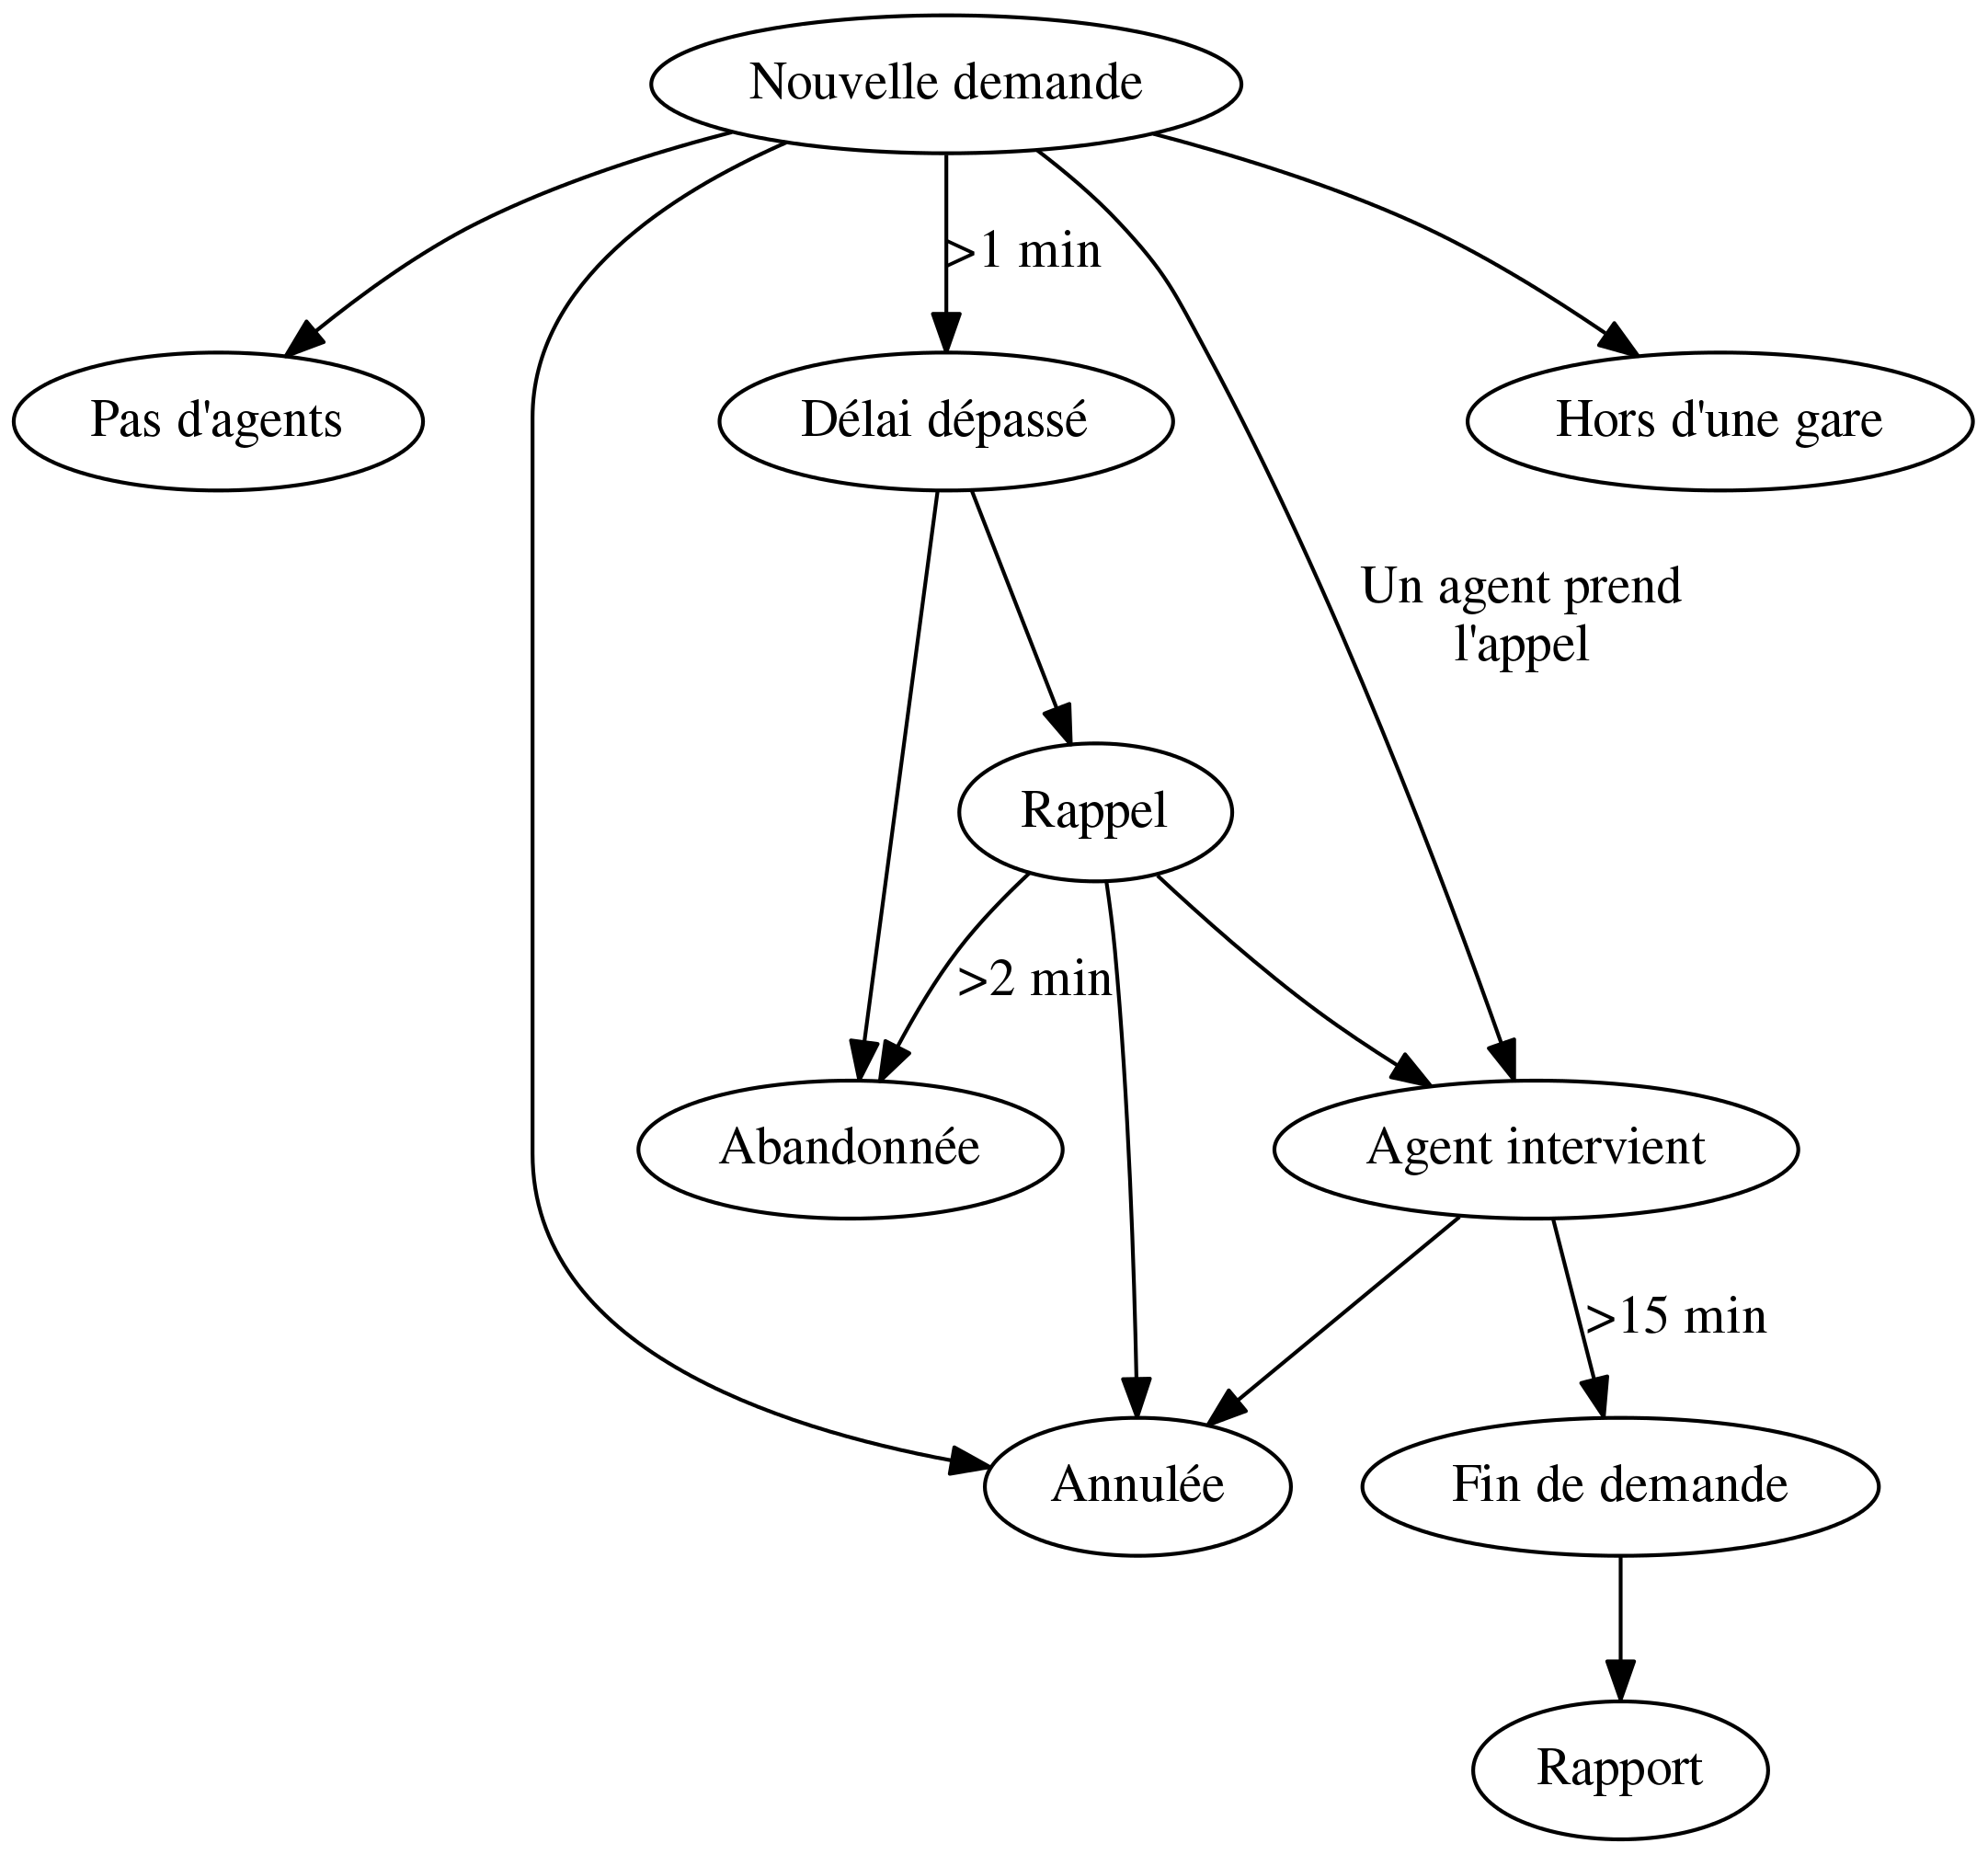
\includegraphics[width=0.8\textwidth]{requete.png}
    \end{centering}
\end{frame}
 
\begin{frame}{Le profil}{Usager}
    \begin{itemize}
        \item Nom
        \item Photo
        \item Téléphone
        \item Téléphone secondaire
        \item Informations complémentaires
        \item Handicap (sélection, 10 choix)
            \begin{small}
                \begin{block}{}
                    \begin{columns}
                        \begin{column}{0.5\textwidth}
                            \begin{itemize}
                                \item Non précisé
                                \item Moteur - fauteuil manuel
                                \item Moteur - fauteuil électrique
                                \item Moteur - marche difficile
                            \item Visuel - aveugle
                        \end{itemize}
                    \end{column}
                    \begin{column}{0.5\textwidth}
                        \begin{itemize}
                            \item Visuel - malvoyant
                            \item Auditif - Téléphone possible
                            \item Auditif - SMS uniquement
                            \item Mental
                            \item Autre
                        \end{itemize}
                    \end{column}
                \end{columns}
            \end{block}
        \end{small}
        \item Handicap (champ libre)
    \end{itemize}
\end{frame}
\begin{frame}{Le profil}{Agent}
    \begin{itemize}
        \item Nom
        \item Identifiant SNCF
        \item (Gares de rattachement)
    \end{itemize}
\end{frame}
\subsection{Spécifications visuelles}
\begin{frame}{L'évolution de l'interface utilisateur}{Équipe HackcessAngels, Janvier-Avril 2014}
    \begin{columns}
        \begin{column}{0.45\textwidth}
            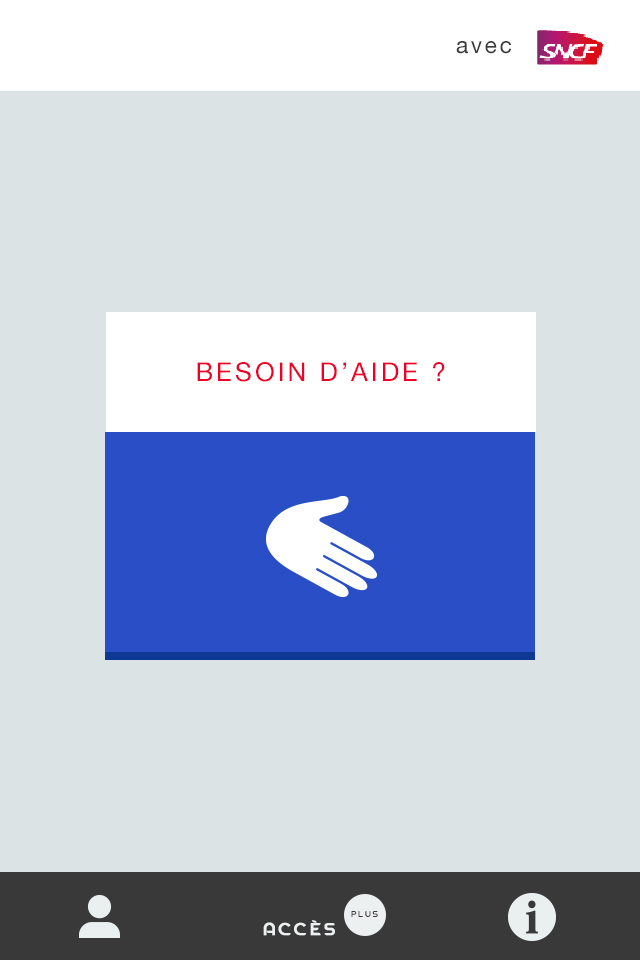
\includegraphics[width=\textwidth]{alex-02/01-home_helpme.jpg}
        \end{column}
        \begin{column}{0.45\textwidth}
            
\includegraphics[width=\textwidth]{alex-02/02-encours.jpg}
        \end{column}
    \end{columns}
\end{frame}
\begin{frame}{L'évolution de l'interface utilisateur}{Expert FiveByFive, Avril-Mai 2014, présenté aux associations}
    \begin{columns}
        \begin{column}{0.45\textwidth}
            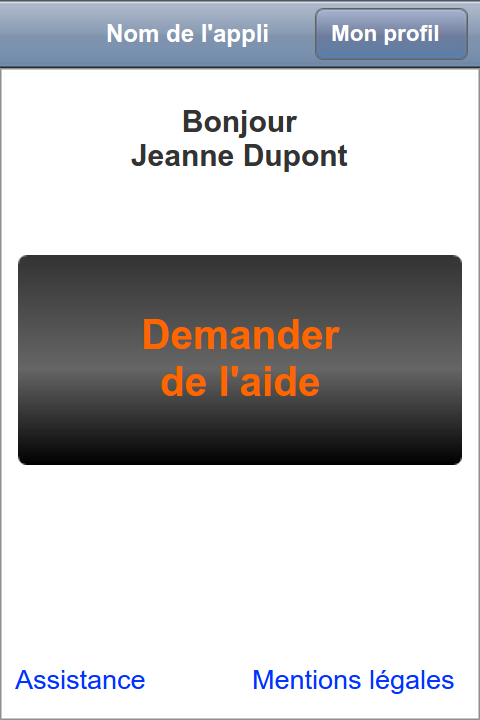
\includegraphics[width=\textwidth]{judith-03/01-home.png}
        \end{column}
        \begin{column}{0.45\textwidth}
            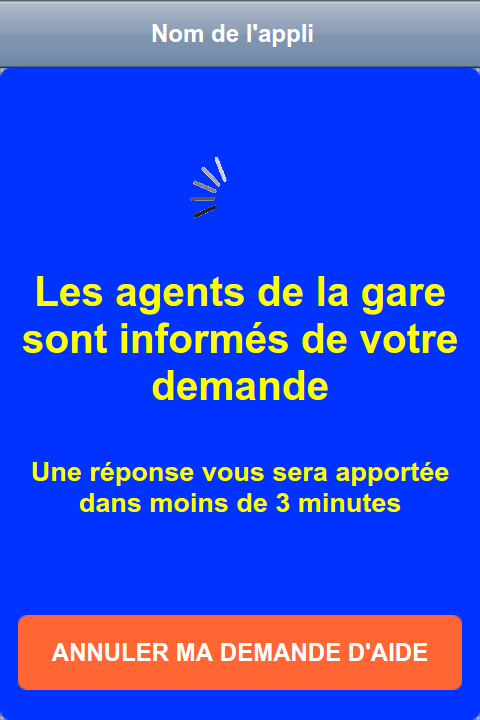
\includegraphics[width=\textwidth]{judith-03/02-encours.png}
        \end{column}
    \end{columns}
\end{frame}
\begin{frame}{L'évolution de l'interface utilisateur}{Designer TwentyFirst, Mai 2014}
    \begin{columns}
        \begin{column}{0.45\textwidth}
            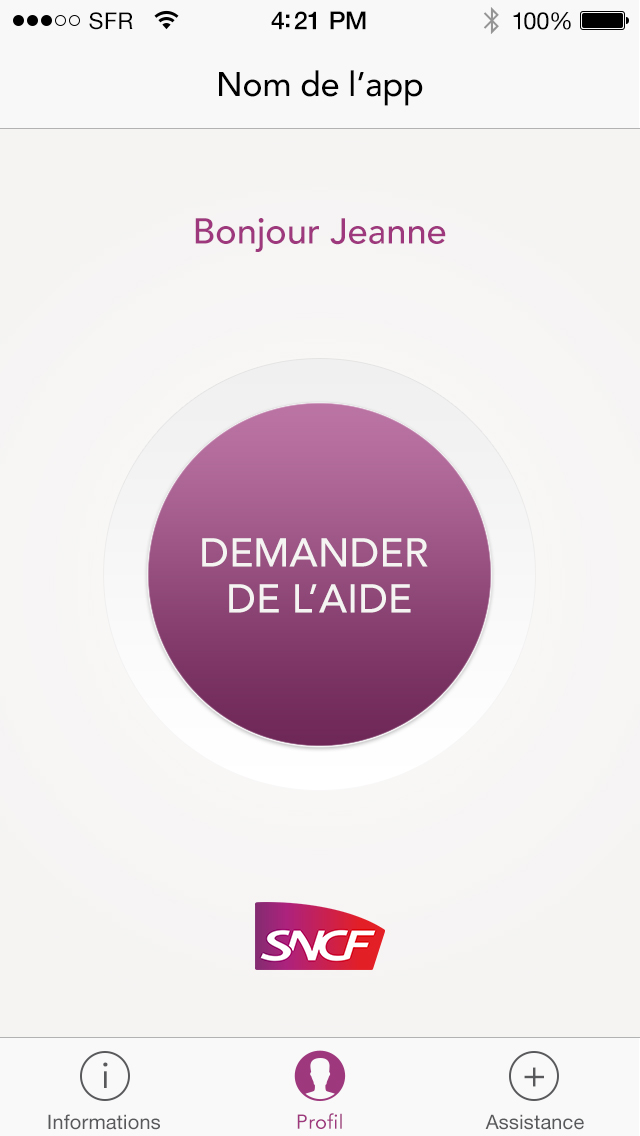
\includegraphics[width=\textwidth]{thibault-04/01-home.jpg}
        \end{column}
        \begin{column}{0.45\textwidth}
            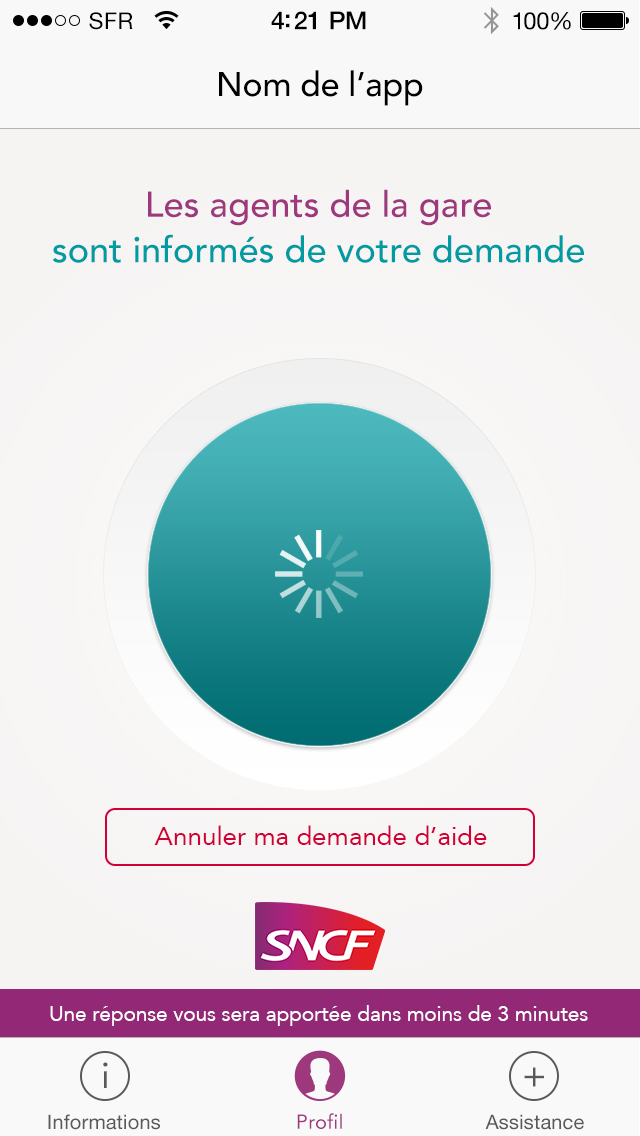
\includegraphics[width=\textwidth]{thibault-04/02-encours.jpg}
        \end{column}
    \end{columns}
\end{frame}
\section{Implémentation}
\subsection{Contraintes}
\begin{frame}{Contrainte \no1: le temps}
    \begin{itemize}
        \item 3 développeurs (1 ingé pro, 2 étudiants)
        \item Le soir et les week-ends
    \end{itemize}
    \begin{description}
        \item[15 mai] Définition des points clefs de l'app (écrans, profils, cycle de vie)
        \item[30 juin] Livraison
        \item[14 jours] Temps de développement "effectif"
    \end{description}
\end{frame}
\begin{frame}{Le matériel}
	\begin{itemize}
		\item 3 dévelopeurs
		\item 2 Macs (1 macbook, 1 mac mini sans écran)
		\item 1 iPhone
	\end{itemize}

	$\Leftarrow$ Quasi-entièrement développé sur simulateur, tests réels impossibles
\end{frame}
\begin{frame}{Les fonctionnalités}
    \begin{itemize}
        \item Profil usager, profil agent, cycle de vie de la demande d'aide : complexe, mais pas compliqué
        \item Cartographie: OpenStreetMap, plug-and-play
        \item Géolocalisations: APIs iOS
        \item "Temps réel": pousser les demandes d'aides vers les agents
            \begin{itemize}
                \item Notifications Apple Push pas fiables
                \item Solution: socket ouvert en permanance (keep-alive 5min)
                \item Interdit dans l'App Store, mais les agents ont leur propre appli interne
            \end{itemize}
    \end{itemize}
\end{frame}
\subsection{Démonstration}
\begin{frame}{Vue d'ensemble}
    Démonstration vidéo
\end{frame}
\begin{frame}{Vue d'ensemble}
    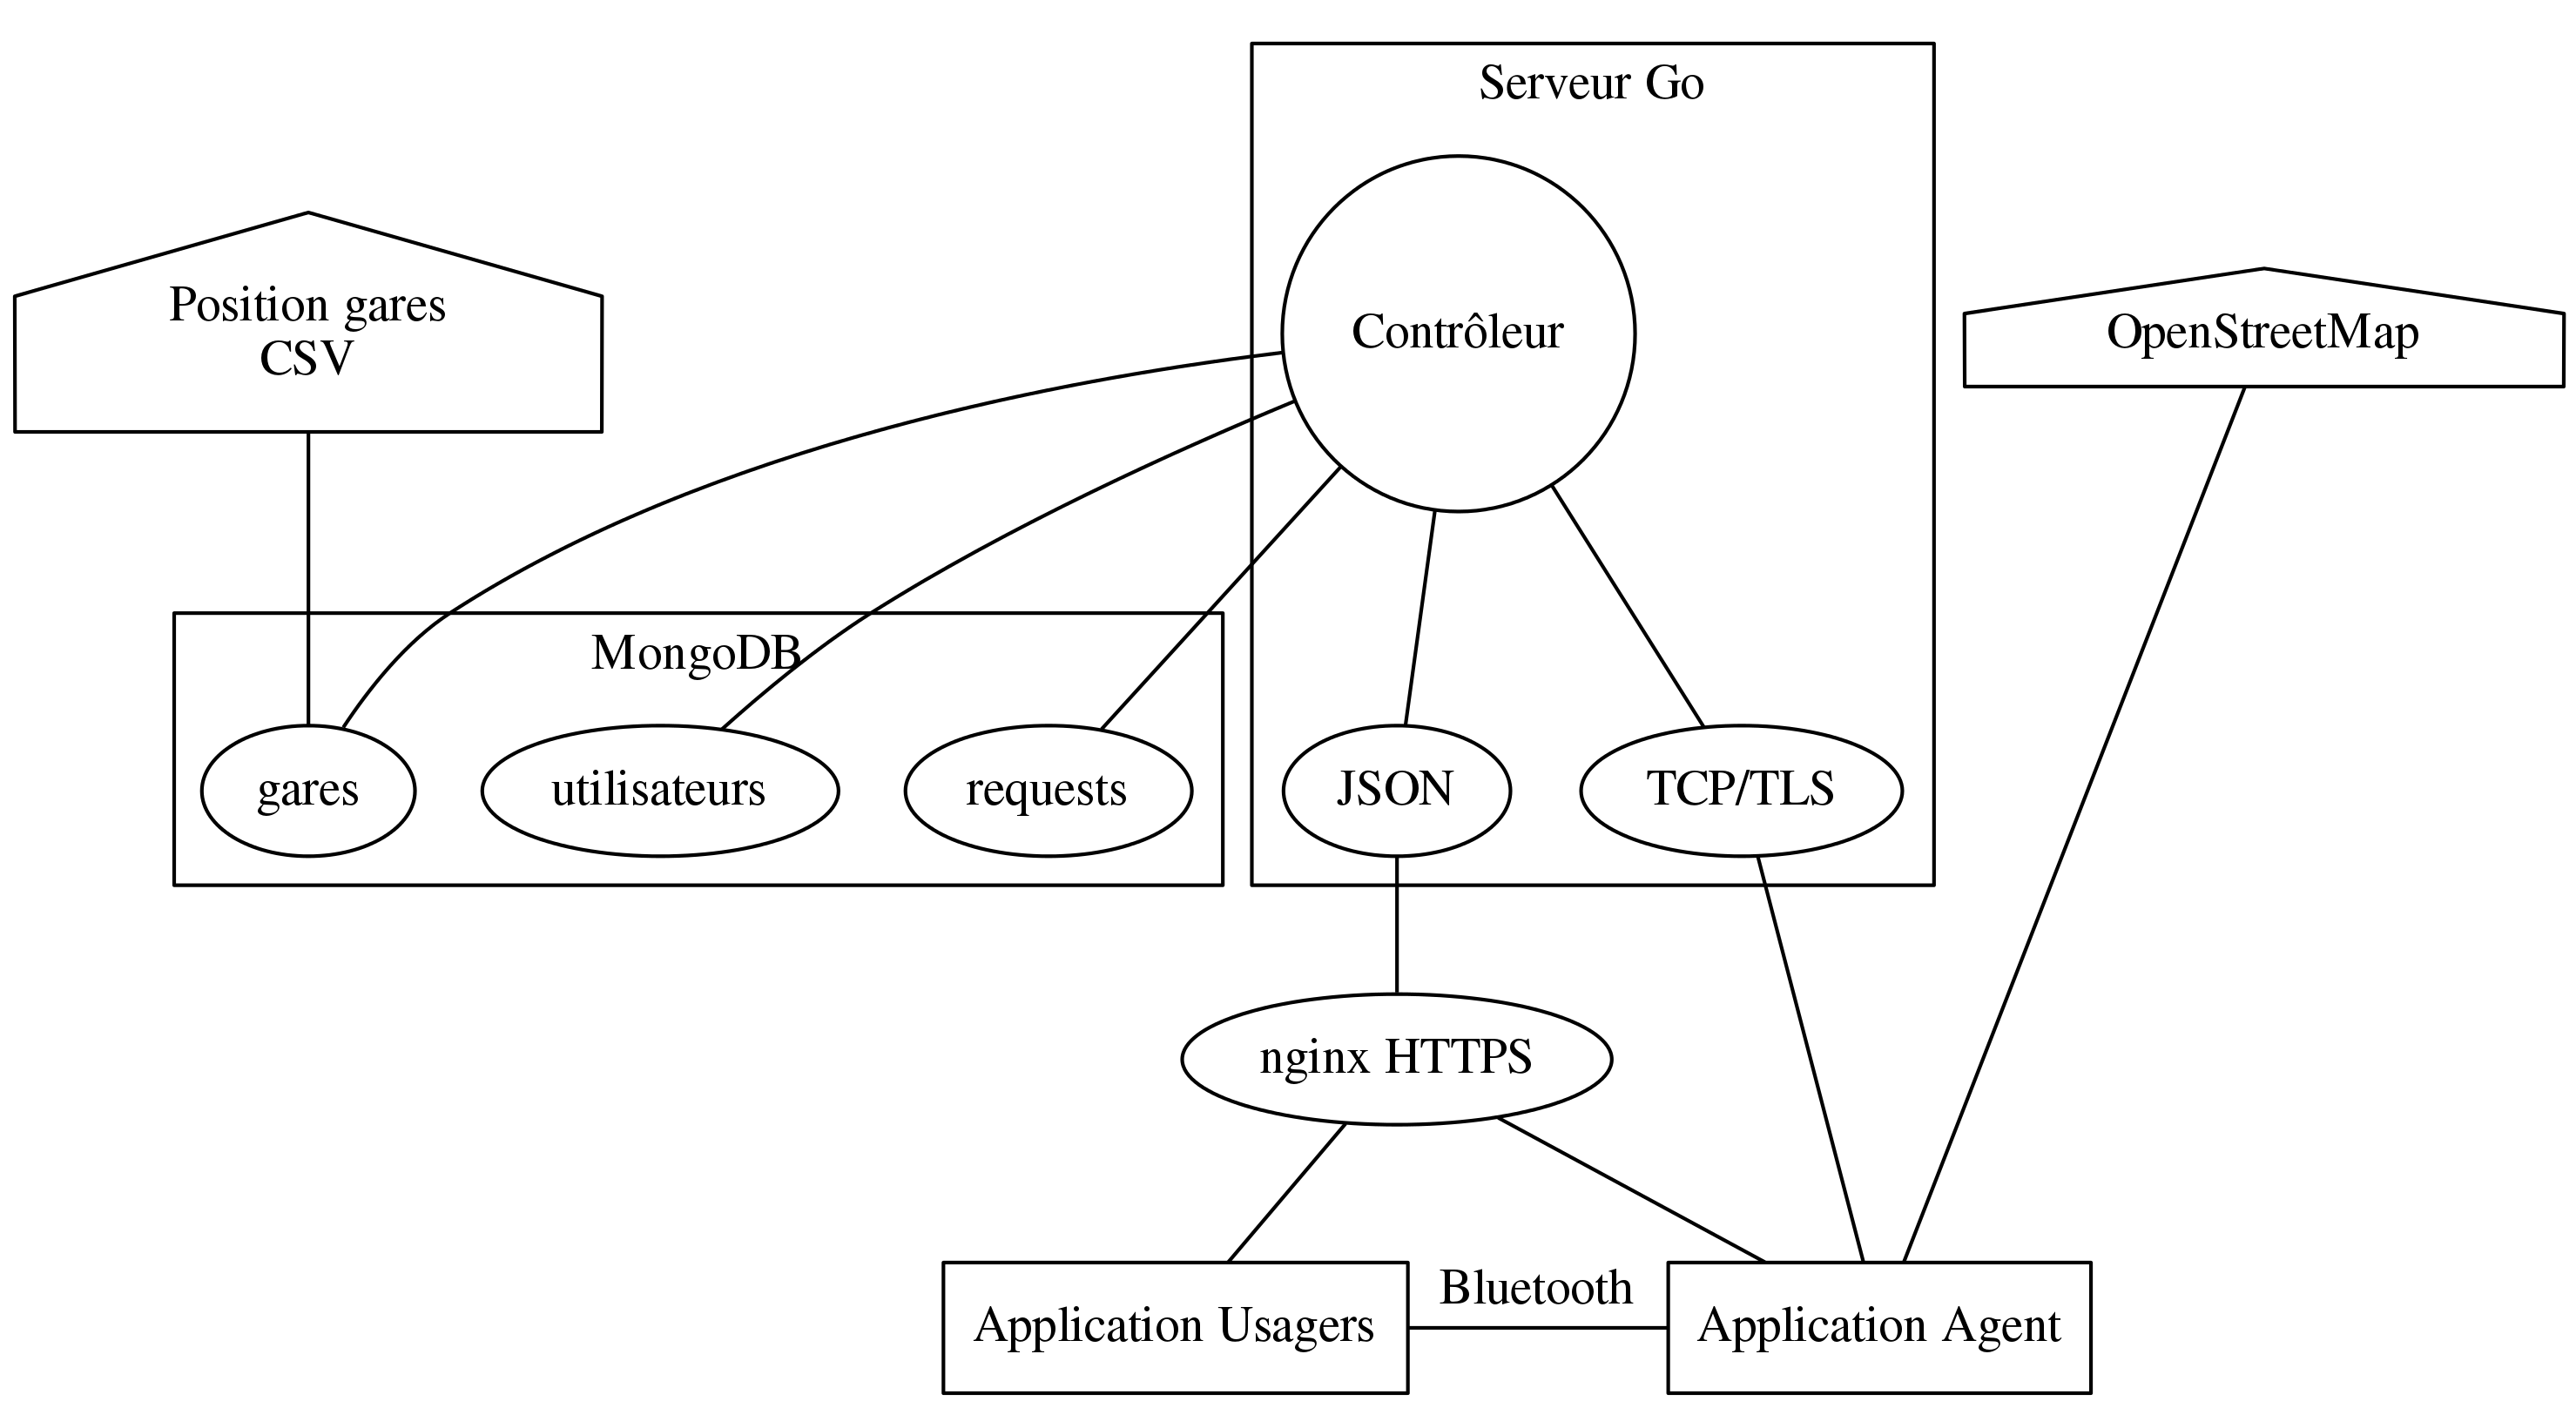
\includegraphics[width=0.8\textwidth]{general.png}
\end{frame}
\subsection{Le serveur}
\begin{frame}{Serveur}
    \begin{itemize}
        \item Gère les profils + demande d'aide sans bluetooth
        \item Go + MongoDB : par familiarité, mais aurait pû être fait avec tout langage
            \begin{itemize}
                \item Index 2D sur les positions des gares
            \end{itemize}
    \end{itemize}
    \begin{block}{Les composants}
        \begin{itemize}
            \item Contrôleur sur BDD MongoDB
            \item API JSON pour les 2 applis
            \item Service TCP vers Aide'Gare agents: liste des agents par gare
            \item Proxy inverse nginx
        \end{itemize}
    \end{block}
\end{frame}
\subsection{Applications}
\begin{frame}{Les applications}
    Structure MVC, avec modèle en commun
    \begin{columns}
        \begin{column}{0.5\textwidth}
            \begin{block}{Usager}
                \begin{itemize}
                    \item Profil dans la keychain
                    \item Utilise l'API JSON pour tout
                    \item BLE: peripheral; advertise quand appel à l'aide
                    \item Internet par défaut
                \end{itemize}
            \end{block}
        \end{column}
        \begin{column}{0.5\textwidth}
            \begin{block}{Agent}
                \begin{itemize}
                    \item Utilise l'API JSON pour profil, données d'appel à l'aide
                    \item Service pseudo-"VoIP": socket TCP/TLS
                    \item socket: pings et gare actuelle
                    \item BLE: central manager
                \end{itemize}
            \end{block}
        \end{column}
    \end{columns}
\end{frame}
\subsection{Suite et fin}
\begin{frame}{Peut-on mieux faire?}{Oui!}
    \begin{itemize}
        \item Remplacer HTTP+socket par service de messaging (0MQ, nanomsg, RabbitMQ)
        \item Meilleur hand-off entre bluetooth et wifi
        \item Extensivité
    \end{itemize}
\end{frame}
\begin{frame}{Les tests en gare}
    \begin{itemize}
        \item Prévus sur 2 semaines (début juillet): 2 gares, usagers et agents sélectionnés
        \item Semaine 1 "libre", semaine 2 observée
        \item Semaine 1: La SNCF et FiveByFive apprennent à utiliser TestFlight
        \item Semaine 2: Des tests internes le lundi, puis plus rien sur le serveur\\
        \item Après enquête: tests annulés et reportés
    \end{itemize}
\end{frame}
\begin{frame}{Les tests en gare}{Les problèmes}
    \begin{itemize}
        \item Fiabilité: D'après les logs, sur 39 tests, 32 ont fait le cycle de vie entier
        \item Possibilités d'abus: Mais les usagers sont choisis et observés\dots
        \item Refus des agents: Si un agent se trouve dans l'autre gare de test, avec son téléphone pro, au moment d'un test, son téléphone peut sonner
        \item Produit fini: La SNCF voulait un produit fini clef-en-main
    \end{itemize}
\end{frame}
\end{document}

